\documentclass[12pt]{extarticle}
\usepackage[utf8]{inputenc}
\usepackage{cite}
\usepackage{graphicx}
\usepackage{subfigure}
\usepackage{geometry}
\usepackage[colorlinks,linkcolor=blue]{hyperref}

\geometry{a4paper,scale=0.8}
\usepackage{cite}

\title{Cloud Data Detection and classification, Stat 154, Spring 2019}
\author{Yanran Li (SID:3034487587)  Junho Woo (SID:23867648)}
\date{April 2019}

\begin{document}

\maketitle

\section{Data Collection and Exploration}
\subsection{Summary}

Sensitivity of Earth’s climate to increasing amounts of atmospheric $CO_2$ is a hot-issue in science and political scene. Especially, if Arctic gets warms, its changed distribution and properties of ice- and snow-covered surfaces, atmospheric water vapor, and clouds can potentially lead to further warming of the earth. Clouds in Arctic plays an important role because detecting clouds can measure the sensitivity of the Arctic’s surface air temperature. Therefore, the goal of this project is to explore a cloud detection and to make a cloud-detection model in arctic with the data collected by the MISR sensor from the NASA satellite Terra. The dataset includes three expert label (+1 = cloud, -1 = not cloud, 0 = unlabeled), three features (CORR, SD, Normalized Difference Angular Inded(NDAI)) and five multi-angel sensor data (Radiance angle DF, CF, BF, AF, AN). The model that we have made is going to be used to distinguish the images without the expert label, meaning that it can be used to detect clouds in the Arctic image\cite{yu2008}.  
 
\subsection{Summarize data}

\begin{figure}[htb]
	\centering
	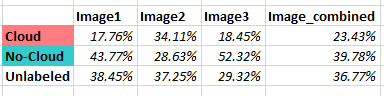
\includegraphics[scale=0.9]{percent.png}
	\caption{$\%$ of pixels for the different classes}\label{fig 1}
\end{figure}

\begin{figure}[htb]
	\centering
	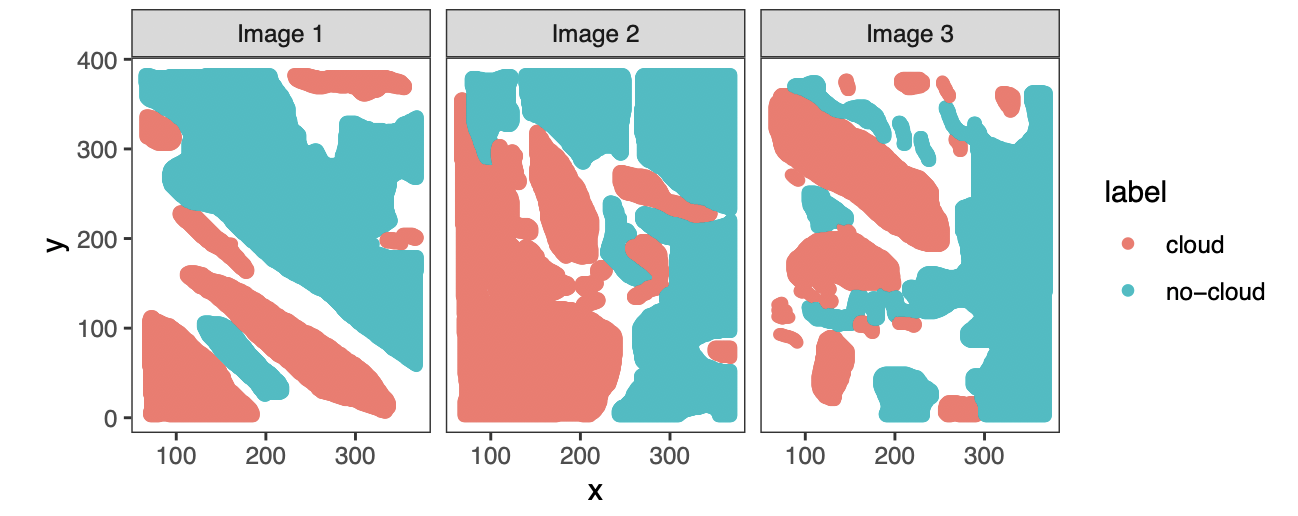
\includegraphics[scale=0.7]{labelEDA.png}
	\caption{expert labels with color of the region}\label{fig 2}
\end{figure}

By looking at  figure 2, we can see that cloud-region and no-cloud region seems to be clustered. Although figure 2 does not explicitly show the trend/pattern, since cloud-region and no-cloud region look clustered(meaning that cloud pixels and no-cloud pixels are not randomly scattered), we can assume the samples justified for this dataset is not i.i.d.

\subsection{EDA}
Pairwise correlation plot (figure 3) shows that NDAI is correlated the most with label (0.76). “CORR” and “SD” are the second and third highest correlation value (0.55, 0.44) with label. To compare individual feature’s value with label, we used boxplot (figure 4). Boxplots shows that values of both x and y coordinates are high at no cloud. For NDAI, SD, and CORR value, cloud data points have higher than no-cloud. Lastly, for angles, no cloud data points have slightly higher value than cloud.




\begin{figure}[htb]
	\centering
	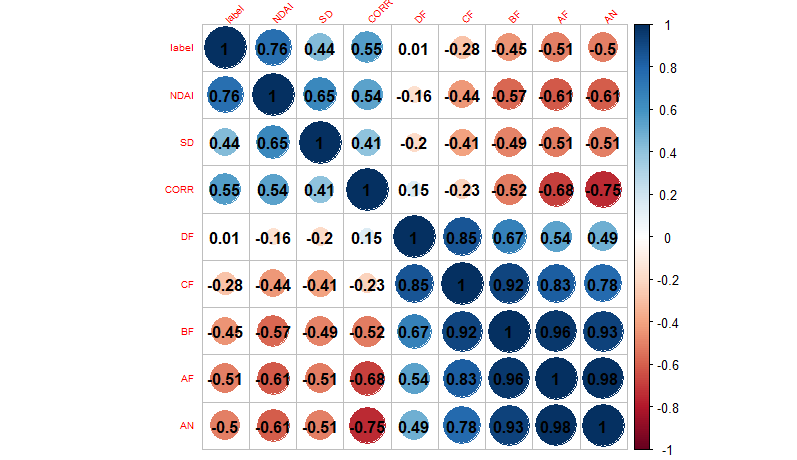
\includegraphics[scale=0.7]{correlation.png}
	\caption{pair-wise relationship of the features}\label{fig 2}
\end{figure}


\begin{figure}[htb]
\centering
\subfigure[boxplot of x and y]{
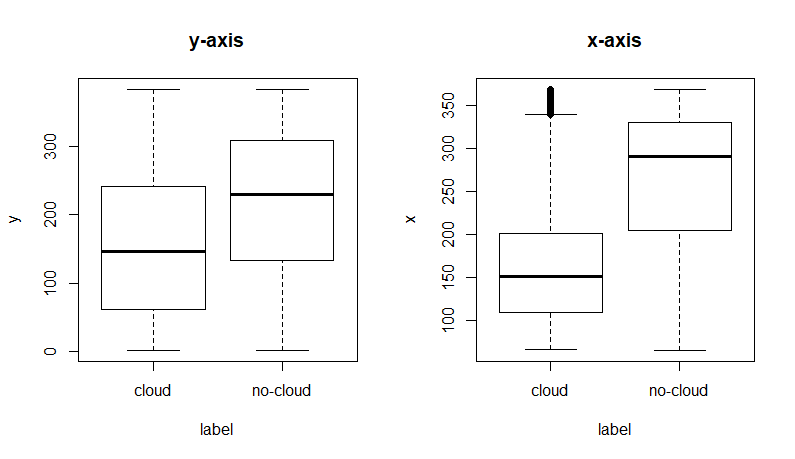
\includegraphics[width=6.0cm]{6.png}
%\caption{fig1}
}
\quad
\subfigure[boxplot of NDAI, SD, CORR]{
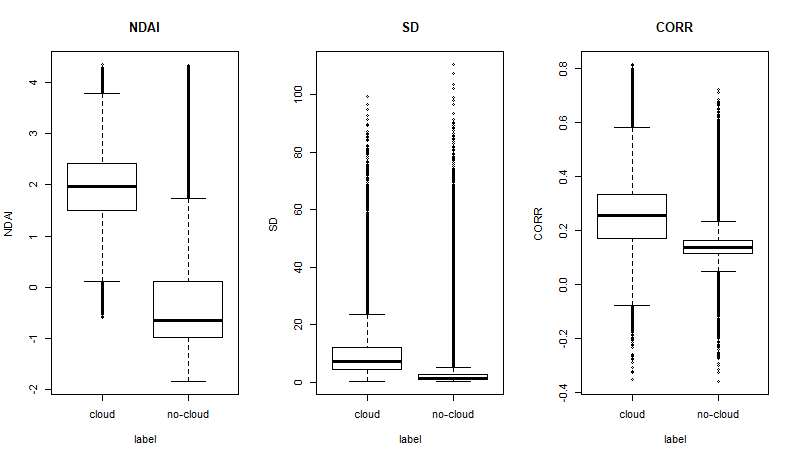
\includegraphics[width=6.0cm]{7.png}
}
\\
\subfigure[boxplot of other features]{
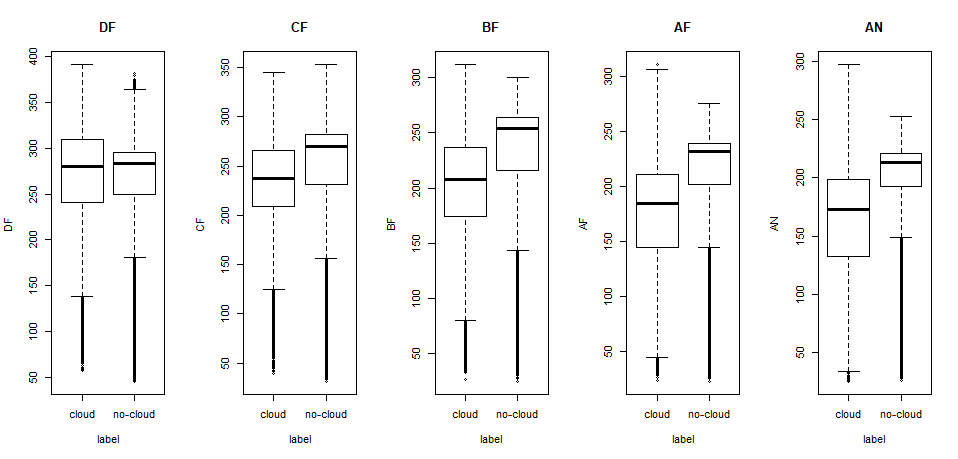
\includegraphics[width=8.0cm]{8.png}
}

\caption{relationship between the expert labels with the individual features.}\label{fig 1}
\end{figure}


\section{Preparation}

\subsection{Split the data}
Before we do modeling, we first Split the entire data into three sets: training, validation and test.
First, we combine the three image data together, remove the unlabeled data (about 40\% of the data are unlabeled) and convert the label to categorical data (+1 = cloud, 0 = not cloud). Then we use 2 ways to split the total image data into training (60\%), validation(20\%) and test (20\%) set.
First, we do randomly sampling(use $sample()$ function in R) to split the data.

As the second non-trivial way, we divided the image in to several grids, and sample grids as training, validation and test set sat each time. In this way, the non-i.i.d data can perform better.

\subsection{Baseline}
Consider the validation and test set, we set all labels to -1 (cloud-free) on them, and we use 2 simple classifier(logistic regression and QDA) to compute the accuracy after training the unchanged training set.The following results are generated by using the average grid sampling method.
\\By using logistic regression, we got the accuracy 59.34\%. By using QDA, we got the accuracy 64.1\%. It does make sense since the ideal test accuracy of i.i.d. data in this case will be 50\%, they are quite close. Only when we have the nearly no-cloud scenario in the test set, we will have high average accuracy. But this doesn't make sense, we certainly have cloud and no-cloud data commonly exist.

\subsection{First order importance about features}

\begin{figure}[htb]
\centering
\subfigure[NDAI]{
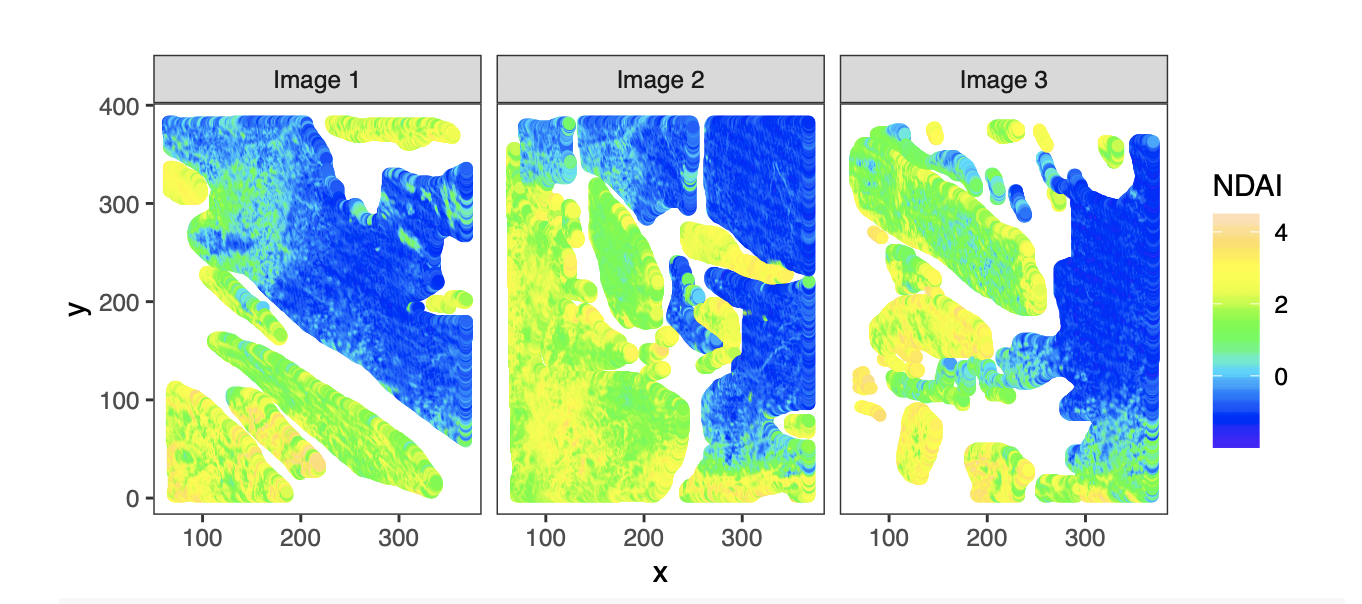
\includegraphics[width=8.0cm]{NDAIEDA.png}
%\caption{fig1}
}
\\
\subfigure[CORR]{
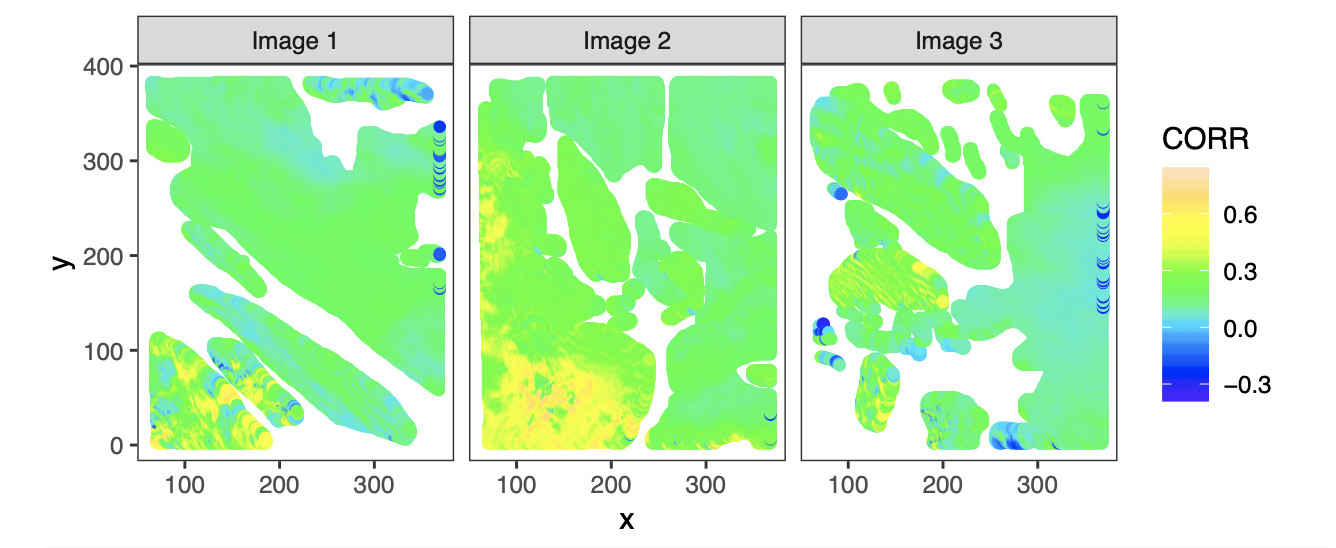
\includegraphics[width=8.0cm]{CORR.png}
}
\\
\subfigure[SD]{
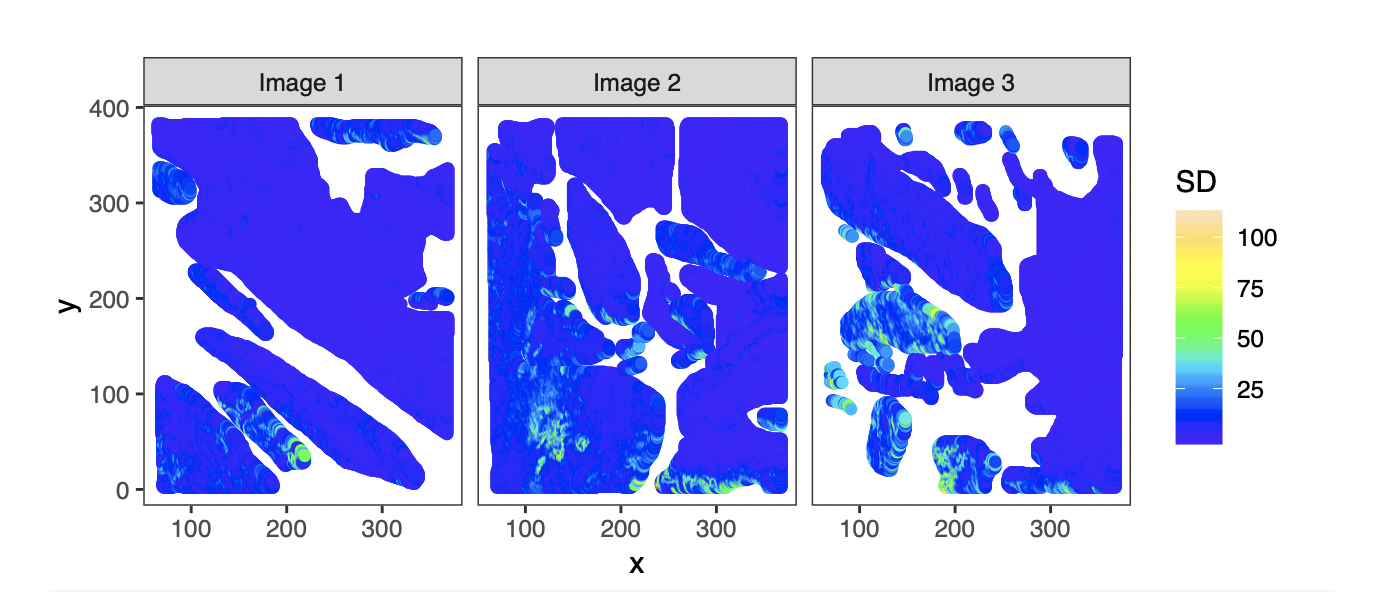
\includegraphics[width=8.0cm]{SD.png}
}

\caption{features' EDA}\label{fig 1}
\end{figure}

NDAI, SD, and CORR are the best features to construct a model. First, as we have seen in figure 3, NDAI, CORR, SD are ones highly correlated with label(0.76,0.55,0.44). In figure 5a, we can see that NDAI value above 0 indicates cloud-ness and NDAI value close to 0 and below 0 indicates no-cloud. Figure 5b and 5c show that CORR and SD are not good indicator of cloud-ness but it is possible to say that high CORR values most likely lie on cloud-region. For figure 5c, we can say that no-cloud area has low SD.  Figure 6 shows density functions of features along with label. With this density functions of features, we can check our three best features are better than others (NDAI, CORR, and SD). The reason we chose NDAI, SD, and CORR are the best features for classification is that we can set distinguishable value (threshold) between cloud and no-cloud. For example, most no-cloud NDAI values will lie between -2 and 0. For SD, although this is as good as NDAI, we can still assume that really low value of SD indicates no-cloud. For CORR, again, this is not as good as NDAI, but still, we can assume that CORR more than 2.5 would be cloud. 

\begin{figure}[htb]
	\centering
	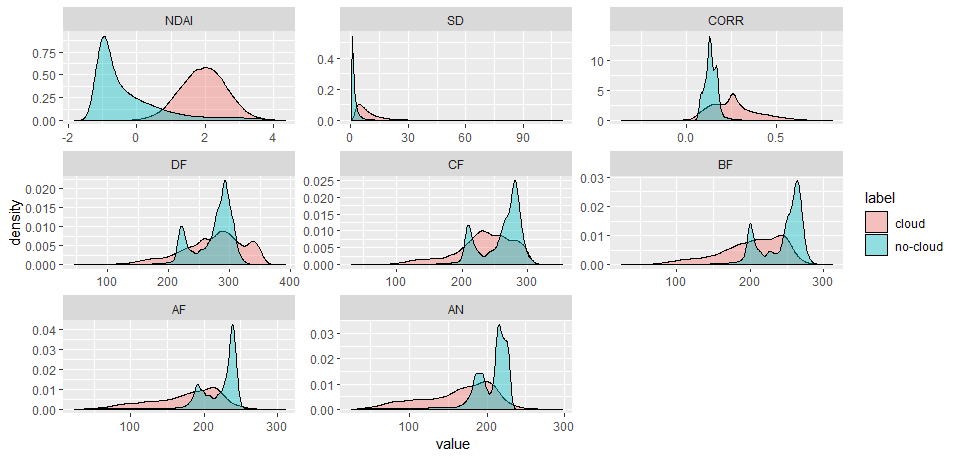
\includegraphics[scale=0.7]{density.PNG}
	\caption{density functions on the features}\label{fig 2}
\end{figure}



\section{Modeling}
\subsection{Several classification methods using cross validation}
\subsubsection{ Logistic Regression}
Logistic regression is a widely-used discriminative classification method which models the conditional distribution of the outcome given the covariates as a Bernoulli random variable with success probability given by the logistic function evaluated at $X_i\beta$. Here $X_i$ is the covariate vector and $\beta$ the coefficient vector. It further supposes that the response variables are independent conditioned on the observed features. 

Since we use 2 ways to split the data in 2(a), we have 2 ways to create folds in our cross validation part. 
Meanwhile, we create 10 folds to do the cross validation. The accuracies across folds also the test accuracy generated by 2 ways can be shown by the following:

\cdot \emph{average grid sampling:}

\underline{fitted-model:}
$y=-3.347+1.896\times NDAI-0.074\times SD+8.992\times CORR$

\underline{10-folds’ accuracies:}
0.8953349, 0.8940724, 0.8923290, 0.8901647, 0.8919081, 0.8922688, 0.8907659, 0.8903451, 0.8923290, 0.8959360

\underline{test accuracy:}  $89.32\%$\\

\cdot \emph{randomly sampling}

\underline{fitted-model:}
$y=-3.327 + 1.901\times NDAI - 0.075\times SD +  8.913\times CORR$

\underline{10-folds’ accuracies:}
0.8898040, 0.8912468, 0.8953950, 0.8928700, 0.8927498, 0.8943129, 0.8878802, 0.8944331, 0.8923290,
0.8940123

\underline{test accuracy:}  $ 70.05\%$

\subsubsection{LDA}
Linear discriminant analysis (LDA) for binary classification aims to separate the feature space using a hyperplane.  It assumes that the each class is normally distributed with means $\mu_0$ and $\mu_1$ and that the two classes are homoscedastic with covariance matrix $\Sigma_0=\Sigma_1=\Sigma$. 

\begin{figure}[htb]
\centering
\subfigure[randomly sampling use LDA]{
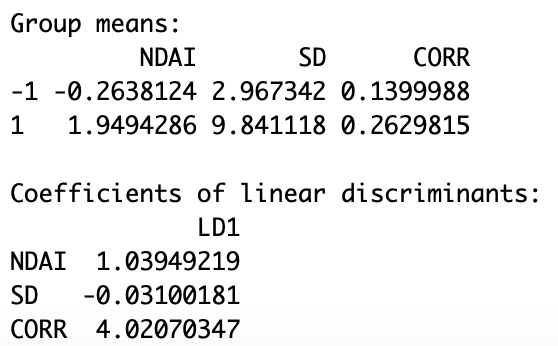
\includegraphics[width=6.0cm]{lda_rand.png}
%\caption{fig1}
}
\quad
\subfigure[average grid sampling use LDA]{
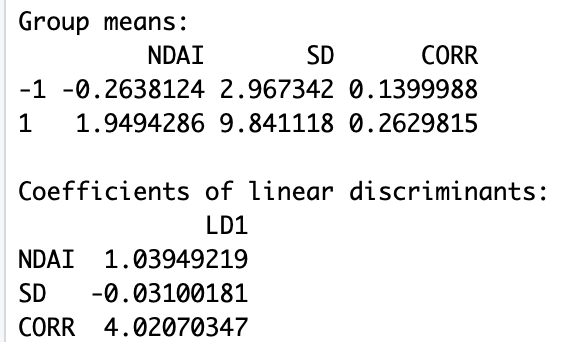
\includegraphics[width=6.0cm]{lda_grid.png}
}

\caption{LDA parameters}\label{fig 1}
\end{figure}

\cdot \emph{average grid sampling:}

\underline{10-folds’ accuracies:}
0.8962598, 0.8944588, 0.8980008, 0.8968602, 0.9004022, 0.8960197, 0.8983549, 0.8987213, 0.8968602, 0.8992015


\underline{test accuracy:}  $89.77\%$\\

\cdot \emph{randomly sampling}

\underline{10-folds’ accuracies:}
0.8993628, 0.9015871, 0.8925093, 0.8961164, 0.9013466, 0.8968378, 0.8946134, 0.8963569, 0.8988818,
0.8967777


\underline{test accuracy:}  $ 69.89\%$

\subsubsection{QDA}
Quadratic discriminant analysis works similiar to LDA except that it makes no assumptions about the covariance matrix.  Thus given the multivariate Guassian distribution:
\begin{equation}
f_c(x) = \frac{1}{(2 \pi)^{p/2} \vert \Sigma_c \vert ^{1/2}} e^{-\frac{1}{2}(x-\mu_c)^T \Sigma_c^{-1} (x-\mu_c)}
\end{equation}
where $c=1,2$ is the class label.


\begin{figure}[htb]
\centering
\subfigure[randomly sampling use QDA]{
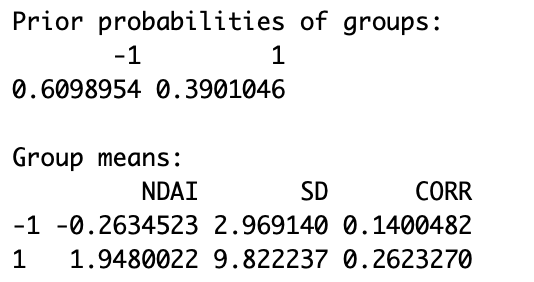
\includegraphics[width=6.0cm]{qda_rand.png}
%\caption{fig1}
}
\quad
\subfigure[average grid sampling use QDA]{
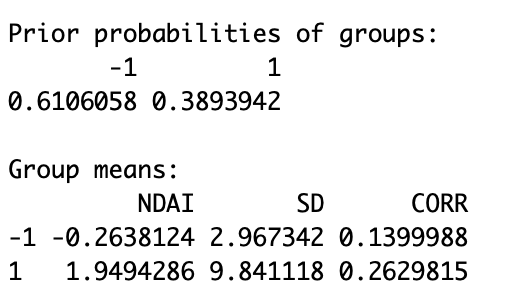
\includegraphics[width=6.0cm]{qda_grid.png}
}



\caption{QDA parameters}\label{fig 1}
\end{figure}

\cdot \emph{average grid sampling:}

\underline{10-folds’ accuracies:}
0.9000420, 0.8956532, 0.8933181, 0.8975206, 0.8970403, 0.8983610, 0.8965000, 0.8976406,
0.8916371, 0.8981209


\underline{test accuracy:}  $89.71\%$\\

\cdot \emph{randomly sampling}

\underline{10-folds’ accuracies:}
0.8979199, 0.8941926, 0.8960563, 0.8958158, 0.8990020, 0.8945533, 0.8982806, 0.8961164, 0.9000842, 0.8951545


\underline{test accuracy:}  $ 69.49\%$

\subsubsection{SVM}
Support Vector Machines (SVMs) is a data classification method that separates data using hyperplanes. One observation about classification is that in the end, if we only care about assigning each data point a class, all we really need to know do is find a “good” decision boundary, and we can skip thinking about the distributions. Support Vector Machines (SVMs) are an attempt to model decision boundaries directly in this spirit.
If we have labeled data with dimension d, SVMs can be used to generate d − 1 dimensional hyperplanes such that the data space is divided into segments and each segment contains only one kind of data.
After running cross validation using the whole dataset, which cost a lot of time
(so only use the average grid sampling), I got the result:\\
\cdot \emph{average grid sampling:}



\underline{10-folds’ accuracies:}
0.9216063, 0.9207647, 0.9194421, 0.9217266, 0.9193219, 0.9214260,
0.9210052, 0.9198629, 0.9183600, 0.9186606



\underline{test accuracy:}  $92.06\%$

\subsubsection{Random Forest}
Random Forest combines multiple trees to form a powerful model. In the process it reduces dimensionality, removes outliers and treats missing values. Here we build 300 decision trees using Random Forest. This model does not have underlying assumptions on the dataset, expect perhaps that bootstrapping our dataset will produce a representative sample.In this model, we trained on the entire dataset with 10 fold validation too.

\cdot \emph{average grid sampling:}

\underline{10-folds’ accuracies:}
0.9129443, 0.9166166, 0.9191931, 0.9172120, 0.9220101, 0.9157711, 0.9181725, 0.9177523, 0.9197334,
0.9164916


\underline{test accuracy:}  $92.02\%$\\


\begin{figure}
\centering
\subfigure[logistic regression]{
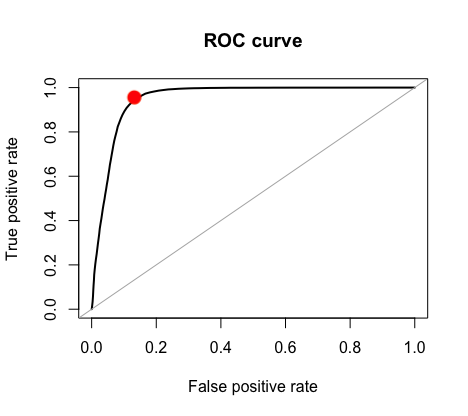
\includegraphics[width=4.0cm]{ROC_lr.png}

}
\quad
\subfigure[LDA]{
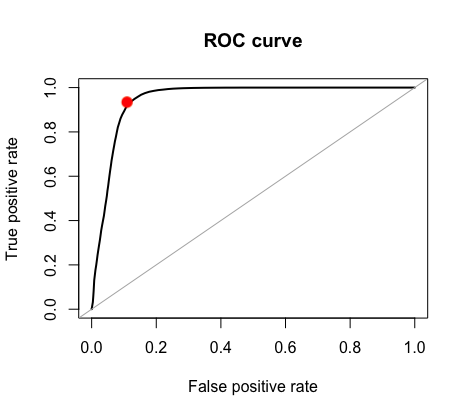
\includegraphics[width=4.0cm]{ROC_lda.png}
}
\quad
\subfigure[QDA]{
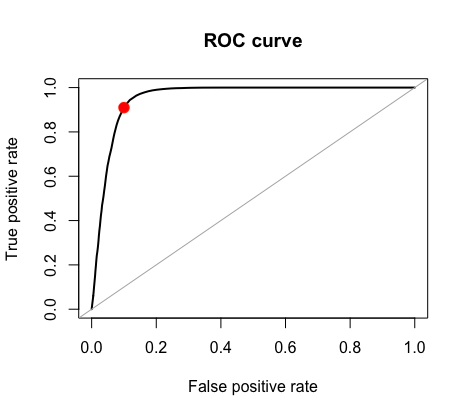
\includegraphics[width=4.0cm]{ROC_qda.png}
}
\\
\subfigure[SVM]{
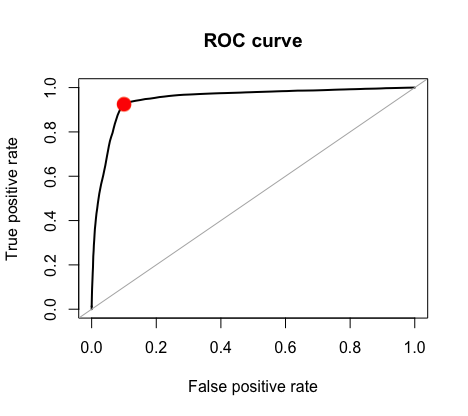
\includegraphics[width=4.0cm]{ROC_svm.png}
}
\quad
\subfigure[random forest]{
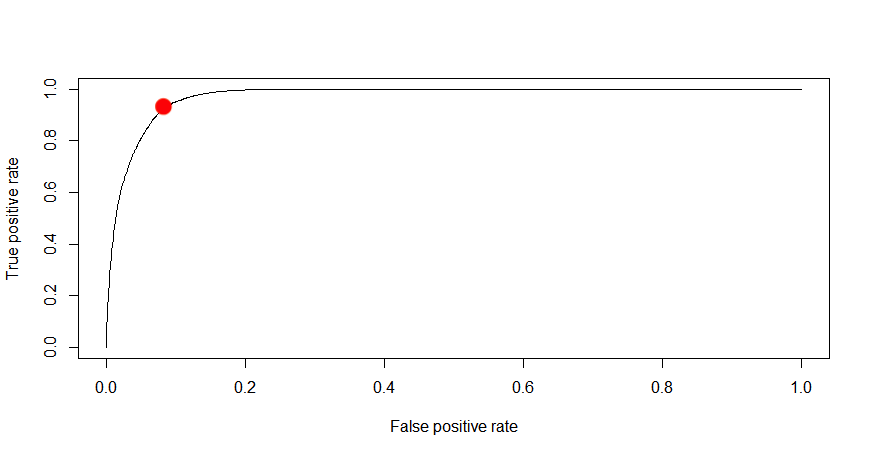
\includegraphics[width=6.0cm]{ROC_rf.png}
}
\quad
\subfigure[AUC values of different models]{
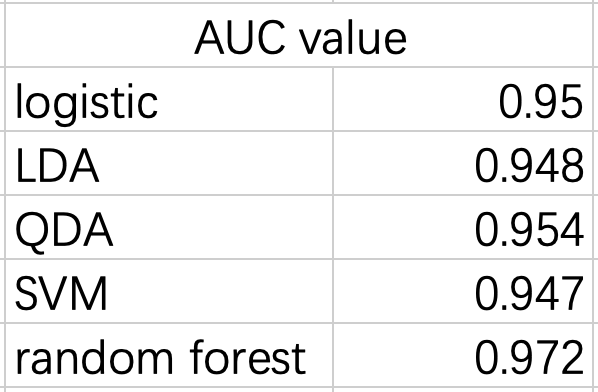
\includegraphics[width=3.0cm]{AUC.png}
}
\caption{5 models' ROC curves and their AUC values}\label{fig 1}
\end{figure}


\subsection{ROC curves}
The results above apparently show that the test accuracy through average grid sampling is exactly higher than the random sampling one, so we use the data split by grid to draw the ROC curves. And then use ROC curves to compare the different models. (See figure9.)

\\We highlight a cutoff value on each of the ROC curves, for which the point on the ROC curve has the minimum distance to the upper left corner. In this case, our cutoff value can make the threshold most closed to the ideal one.
\\By comparing with their AUC values, we can clearly see that the model "random forest" has the highest AUC value, which indicates that the random forest can best distinguish between classes in our cloud data detection.

\subsection{Model Selection}
After comparing the AUC values of our 5 models, the one that random forest got is the highest, so it make sense to choose it as out best classifier in this situation.

In order to choose the best fit model, we also have other methods(model evaluation is done based on testing dataset). The following table shows the detailed measures in confusion matrix, which can also be criterian to measure our models, e.g. $accuracy = \frac{TP+FN}{P+N}, sensitivity = racall = \frac{TP}{P}, specif icity =\frac{TN}{N},precision = \frac{TP}{TP+FP}$. 




\section{Diagnostics}
\subsection{In-depth analysis}
See above, we select random forest as our best classifier. Here are some in-depth analysis about this model.
Seeing the confusion matrix for training CV in rf. It shows that there are 9162 false positive while 4533 was false negative among 166569 training data. To perform Random Forest method, we started with the number of trees = 300 on our training set. Figure10(a)  shows that after trees = 150, there is no significant reduction in error. Since Random forests takes longer than other classifier like LDA, QDA, and Logit, we decided to fix the number of tree = 150 for further use of this random forest method. Figure10(b)  shows the variance important plot. This shows that NDAI $>$ CORR $>$ SD order of importance makes sense when building such model. 
\begin{figure}[htb]
\centering
\subfigure[error rate across decision trees]{
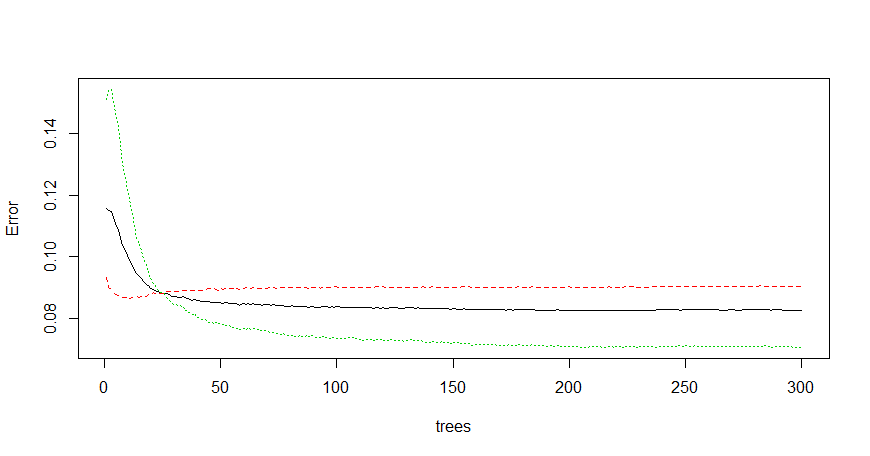
\includegraphics[width=6.0cm]{para_dt.png}

}
\quad
\subfigure[Variable Importance Plot for Random Forest]{
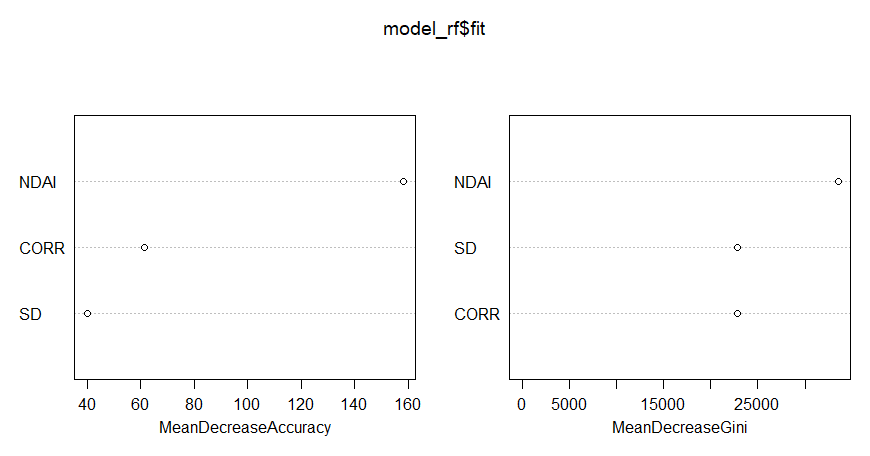
\includegraphics[width=6.0cm]{fig_rf.png}
}
\caption{In-depth analysis on random forest}\label{fig 1}
\end{figure}

\subsection{Misclassification errors}
\begin{figure}[htb]
\centering

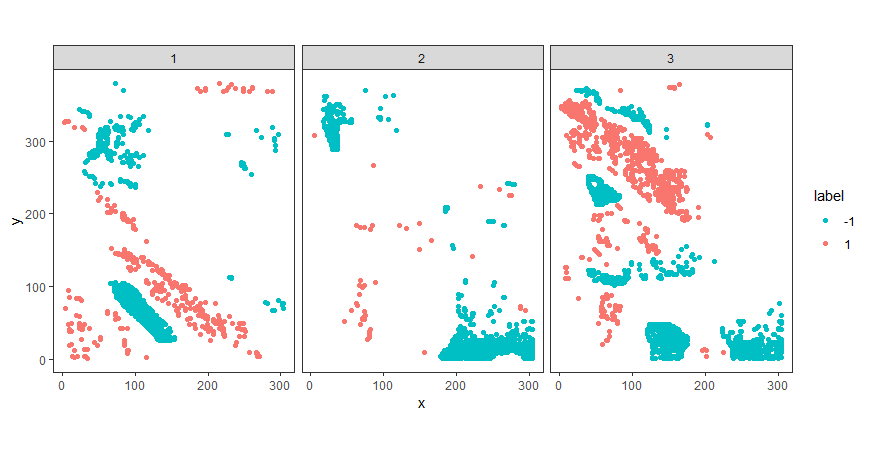
\includegraphics[width=8.0cm]{misclass.png}

\caption{In-depth analysis on random forest}\label{fig 1}
\end{figure}

We used the random forest model to classify test set. The confusion matrix of test data shows 1080 false positive and 2229 false negative. This is made us confusing that on trainning set, we had more “false positive” than “false negative”.  Figure11 is a mis-classification plot. Labeled points in this plot indicate that they were not classified correctly, meaning that red points are supposed to be classified as cloud, but our random forest classification classified it as no-cloud. For image 1 and image 3, misclassification seems to be equally distributed on both cloud and no-cloud. For image 2, we see more blue (no-cloud) points than red(cloud) points, meaning that our model predicted this blue points as cloud(red). Also, we found the pattern that mis-classification tends to happen more on “not-big-clustered region” or edge of the clustered region. It is hard to see misclassification on the middle of a huge clustered region (clouded area or no-cloud area). This pattern makes sense because we didn't split the data randomly to keep spatial correlation, and points that are in the middle of clustered area have neighbors of similar kind, which makes it hard to be misclassified. 
\\
Also, we claimed that the best feature was NDAI: its density function(figure12a) has two distinct gaussian distributions between cloud and no-cloud, which makes us easy to choose the threshold. But NDAI density plot for misclassification data(figure12b) shows that the densities between cloud and no-cloud are mostly overlapped. This implies that since our random forest classification model is built with NDAI, CORR, SD (mainly with NDAI). Therefore, our model would probably misclassify when two densities are overlapped.


\begin{figure}[htb]
\centering
\subfigure[density plot of NDAI in raw data]{
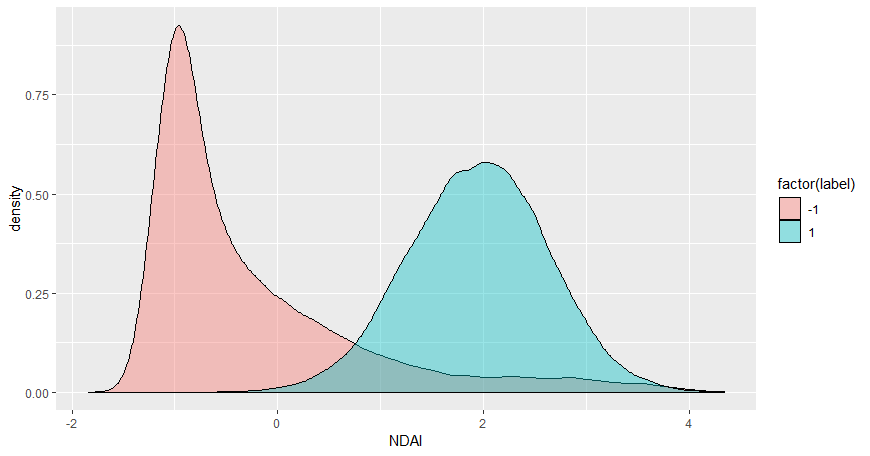
\includegraphics[width=8.0cm]{rawNDAI.png}

}
\quad
\subfigure[density plot of NDAI in misclassification data]{
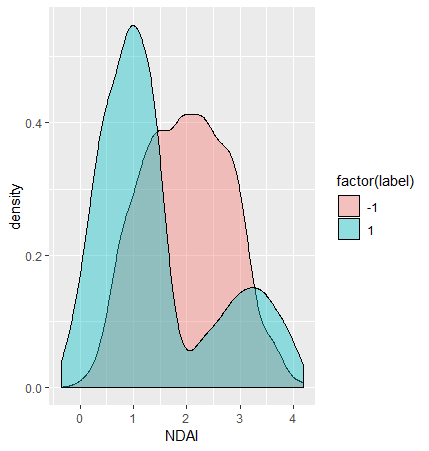
\includegraphics[width=4.0cm]{misclaNDAI.png}
}
\caption{density plots of NDAI}\label{fig 1}
\end{figure}

\subsection{Future work}
Since the original paper mentioned NDAI, CORR, SD are the best features to build classification models, we just followed what the paper stated for previous part. However, 5 angular features would be helpful to build a better classification model, so we decided to add 5 angular features on our random forest model. We ran random forest method, the best classification method we claimed, with additional 5 angular features on grid-splitting. Surprisingly, performance of this method improved. This means that angular features should not be ignored when building classification models. Mean trainCV error is 96.04008\%, which is higher than random forest trained with only 3 features. The accuracy on test data set is, again, higher than 3-feature tested one(96.14\%). 
\\To investigate pattern of misclassification, we plotted the same way we did in part 4(a) and 4(b) and compared them(See figure 13). Seeing the confusion matrix, 9-feature random forest’s misclassification error behaves similarly to the 3-feature one; there are more “false negative” than “false positive”. Figure13a shows the misclassification area. Clearly, 9-feature plot has less misclassified area than 3-feature plot and it looks less dense than 3-feature misclassification plot. We found the pattern that many misclassification points in the middle of misclassification region from 3-feature misclassification plot got disappeared in 9-feature misclassification plot. This means that with additional angular features, misclassified points in the middle of misclassified region can be classified correctly. Lastly, we compared NDAI densities plot. NDAI for 9-feature random forest misclassification density plot has more overlapped region between cloud and no-cloud than 3-feature random forest misclassification density plot. Also the  importance among the 9 features is shown in figure 14, by which we know that $NDAI > SD > CORR > AN> DF> CF> BF >AF$ for feature importance.

\begin{figure}[htb]
\centering
\subfigure[9-feature random forest misclassification plot]{
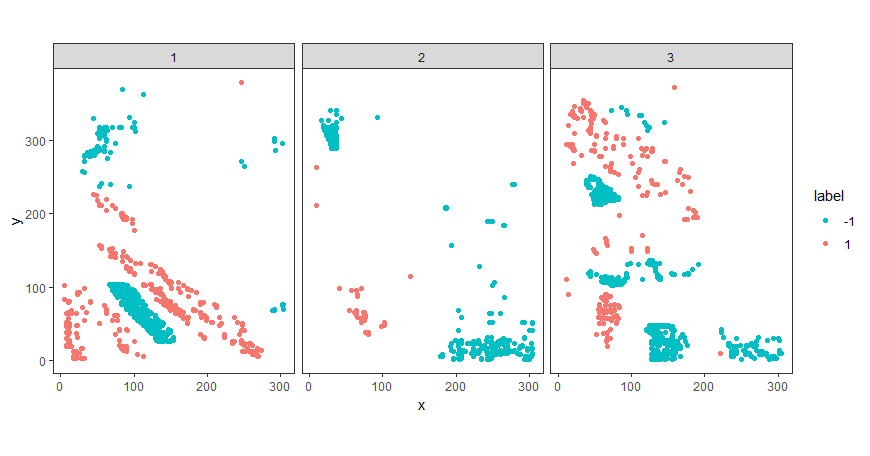
\includegraphics[width=8.0cm]{9mis.png}

}
\quad
\subfigure[9-feature density plot of NDAI in misclassification data]{
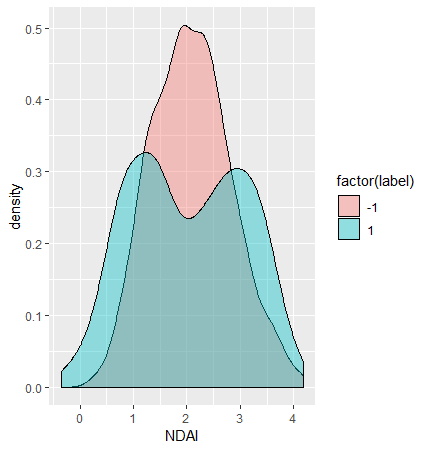
\includegraphics[width=4.0cm]{9ndai.png}
}
\caption{Comparing the misclassification data in 9 features}\label{fig 1}
\end{figure}

\begin{figure}[htb]
	\centering
	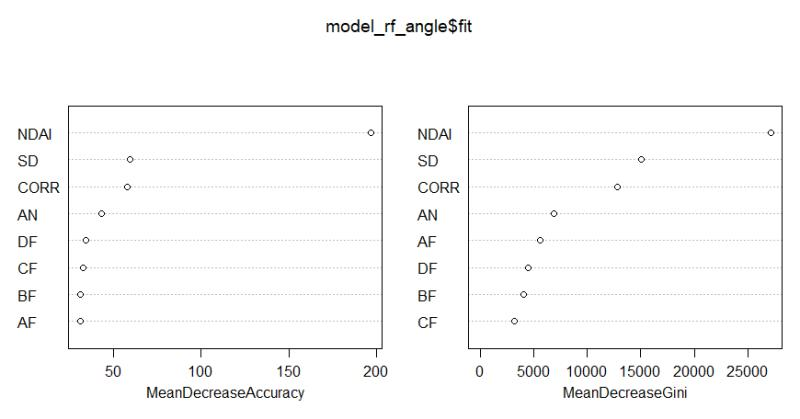
\includegraphics[scale=0.6]{9importance.png}
	\caption{variance importance plot for 9 feature random forest}\label{fig 2}
\end{figure}

\subsection{Diagnostic plots of prediction on unlabeled data}
Here we use our best fit model (Random Forest) to predict the unlabeled observation data and then combine the predicted data with the labeled ones and plot the pixel-level three image data to distinguish clouds from non-clouds, and we compared them with 3 main features and all features. Figure 15 shows the results of classification, compared with Figure 2, we can see that the white part in Figure 1 are classificied as either cloud or no cloud in Figure 15. We can see clear patterns in our figure, which means our classification for unlabeled area are reasonable. In addition, the all-feature one has more clear margin, which means that it may cause some over-fitting problems after using all features to train our model. Maybe choose 3 main features is enough.
\begin{figure}[htb]
\centering
\subfigure[prediction on unlabeled data with 3-feature training]{
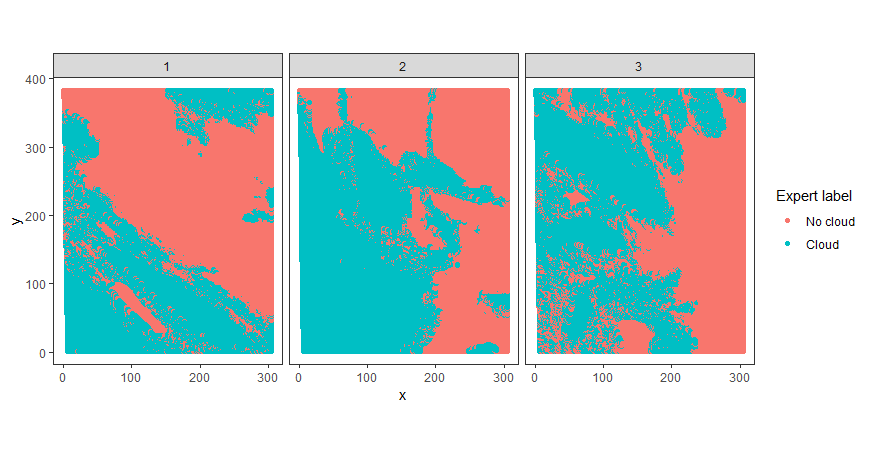
\includegraphics[width=6.0cm]{unlabel3.png}

}
\quad
\subfigure[prediction on unlabeled data with all-feature training]{
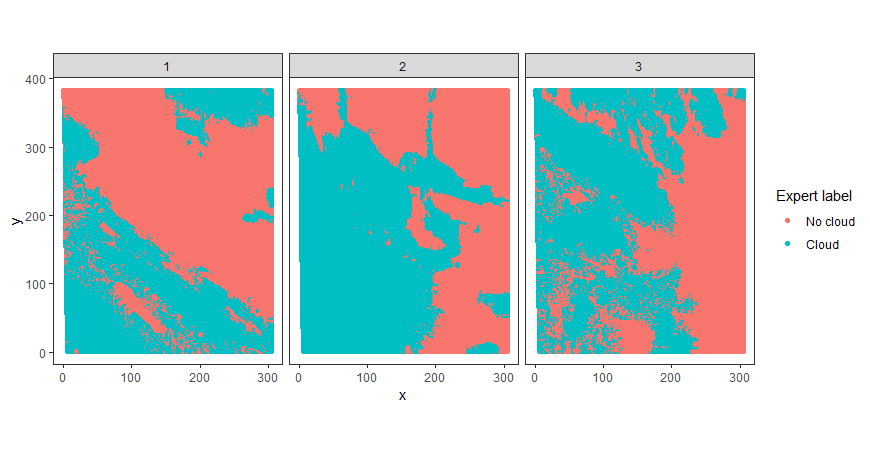
\includegraphics[width=6.0cm]{unlabel4.png}
}
\caption{add prediction on unlabeled data EDA}\label{fig 1}
\end{figure}



\subsection{The way of splitting the data}
After modifying the way of splitting the data (we use the random sampling one), there was not much difference between average-grid-sampling and random sampling through our random forest clssifier, both of which give a high test accuracy values, but for the misclassificaton data plot and also the prediction of unlabelled data, the grid one performed a little bit better. This shows that the non-i.i.d. data need grid-sampling to split the data and then implement the training. However, because our grid-sampling split the image tightly and random forest is such a good classifier, to improve spatial correlation, we should split the image in less parts (like $3\times 3$ or $3\times 4$), after which we would see the difference in result between grid-sampling and random sampling. 








\section{conclusion}

Logistic regression, LDA, QDA, SVM and random forest all created reasonable predictive models with high AUC values.  Each model has some advantages and disadvantages. On average, random forest did best through cross validation. Logit and QDA/LDA have parametric assumptions on the distribution of the classifications, and they are much simpler to compute, but accuracy is not as good as SVM or Random Forest, which are “new” machine learning methods. Our final model, random forest,
only assumes no heavy tails. In the absence of significant domain knowledge, coupled with the better AUC/ROC performance, we are inclined to conclude random forest generalizes better. 


\section{Reproducibility}
Our repository is at \href{https://github.com/Lyric98/STAT-154-Cloud-Classification}{https://github.com/Lyric98/STAT-154-Cloud-Classification}


\section{Acknowledgment}
We read paper and discussed together. Problem 1, 4 are mostly done by Junho Woo and problem 2, 3 are mostly done by Yanran Li. Thanks to GSIs to answer our questions in office hours. Thanks to Jilin Cao, Zhengyi Sui etc. discussing some questions with us together.




\bibliographystyle{plain}
\bibliography{M335}

\end{document}
